%% Documentclass:
\documentclass[manuscript]{stjour}

%% Or,

%% Manuscript, for double spaced, larger fonts
% \documentclass[manuscript]{stjour}
%% Only needed if you use `manuscript' option
\journalname{Open Mind}

%%%%%%%%%%%%%%%%%%%%%%%%%%%%%%%%%%%%%%%%%%%%%%%%%%
%% For production only, not authors:
%%\documentclass[OpenMind,finalfonts]{stjour}

%%%%%%%%%%% Please supply information %%%%%%%%%%%%%%%%%%%%%%%%%

%% For Open Mind:
%% Supplementary Materials:
\supplementslinks{dx.doi.org/10.1098/rsif.2013.0969}

%% If no conflicts, this command doesn't need to be used
%% \conflictsofinterest{}

%%%%%%%%%%% to be supplied by MIT Press, only %%%%%%%%%%%%%%%%%

\citation{Niyogi, R. K., Breton, Y.-A., Solomon,
R. B., Conover, K.,\\ Shizgal, P., Dayan, P. (2015).\\ 
Optimal indolence: a normative microscopic approach to work and leisure. Open Mind 1(1):
1−12.}

\received{XXX}
\accepted{XXX}
\published{XXX}

%% DOI address:
\setdoi{10.1098/rsif.2013.0969}

%%%%%%%% End MIT Press commands %%%%%%%%%%

%%%%%%%%%%%%%%%%%%%%%%%%%%%%%%%%%%%%%%%%%%%%%%%%%%%%%%%%%%%%%%%
%% author definitions should be placed here:

%% example definition
\def\taupav{\tau_{\mathrm{Pav}}}
\usepackage{todonotes}
\begin{document}

\title{The pragmatics of perspective-taking}
\subtitle{Gricean expectations account for apparent limits on theory of mind use}

%% If shortened title for running head is needed so that the article title can fit
%%   in the running head, use [] argument, ie,
%%
%%   \title[Shortened Title for Running Head]{Title of Article}
%%   \subtitle{Subtitle Here}

%% Since we use \affil{} in the argument of the \author command, we
%% need to supply another version of the author names, without \affil{}
%% to be used for running heads:

\author[Hawkins, Gweon, Goodman]
{Robert Hawkins\affil{1}, Hyowon Gweon\affil{1}, Noah Goodman\thanks{asdf}\affil{1}}

\affiliation{1}{Department of Psychology, Stanford University, Stanford, CA, US}

%ie.
%\affiliation{1}{Gatsby Computational Neuroscience Unit, University
%College London, London, United Kingdom} 

%\affiliation{2}{Another Department, Institution, City, Country}

%ie
%\affiliation{2}{Center for Studies in
%Behavioral Neurobiology, Concordia University, Montreal, Quebec,
%Canada}

\correspondingauthor{Robert Hawkins}{rxdh@stanford.edu}

% ie,
%\correspondingauthor{Ritwik K. Niyogi}{ritwik.niyogi@gatsby.ucl.ac.uk}

\keywords{theory of mind, pragmatics, interaction, communication, social cognition, replication}

%ie
%\keywords{work, leisure, normative, microscopic,  reinforcement learning, economics}

\begin{abstract}
%To communicate successfully, speakers must flexibly adapt %the specificity of 
%their utterances to the demands of the current context. When they are unsure exactly which objects are in view of their partner, for example, they may provide additional disambiguating information when referring to a particular object: saying "cassette tape" instead of the potentially ambiguous ``tape."
Recent debates over theory of mind use have hinged on behavior in natural-language communication tasks but have largely neglected the nuanced pragmatics of these tasks. Under Gricean expectations of cooperativity, speakers ought to be more informative in contexts with high uncertainty about what is in the listener's field of view. If pragmatic reasoning is truly grounded in theory of mind,   A careful analysis of pragmatic demands using a rational model of communication suggests a minimal pair of experiments which show that apparent failures of visual perspective-taking are in fact successes for sophisticated social reasoning in context.
%Recent theories of language use as recursive social reasoning remain in tension with evidence that adult listeners apparently fail to take their partner's perspective in communication. To reconcile these points of view, we use a computational model of communication under uncertainty to analyze the pragmatic demands of a common theory of mind test.  Through a minimal pair of replications comparing scripted vs. unscripted speakers, we show that scripted confederates used in previous studies are \emph{uncooperative}: they are less informative than what a speaker would actually produce in that situation, thus violating the listener's rational social expectations. This ironically shows that apparent failures of theory of mind are in fact attributable to sophisticated expectations about speaker behavior---that is, to theory of mind. 
\end{abstract}

\section{Introduction}\label{introduction}

%%% Characterize the computational approach to theory of mind we plan to take
%%% Point out a gaping hole that could benefit from this approach
Our success as a cooperative species depends upon our ability to make sense of other agents. 
One solution is to maintain an internal predictive model of other agents: how unobservable beliefs and desires give rise to observable actions. 
Such a model allows us to make inferences about a social partner's likely internal state given their past behavior and form sophisticated expectations about their future behavior. 
%This theoretical approach to social cognition, where theory of mind reasoning \cite{PremackWoodruff78_ChimpanzeeToM, GopnikWellman92_TheoryTheory, WellmanCrossWatson01_ToMMetaAnalysis, SetohScottBaillargeon16_FalseBelief, ScottBaillargeon17_EarlyToM} is grounded in an explicit computational model of how other minds work, has 
% The approach has been useful for understanding a number of experimental phenomena in both adults and children \cite{KileyHamlinEtAl13_MentalisticCoreSocial, PantelisEtAl14_IntentionInference, BakerSaxeTenenbaum09_ActionUnderstandingInversePlanning, JaraEttingerEtAl16_NaiveUtilityCalculus, BakerEtAl17_ToMBayesian}. 
Yet our current understanding of theory of mind use in \emph{communication} remains limited. 
Just as making sense of an agent's physical movements in the world requires an accurate model of how beliefs and intentions translate into motor plans, making sense of language depends on an accurate model of what a speaker would say, or what a listener would think, in different situations. 

%While these failures are compelling evidence against a simple model where theory of mind reasoning is limited to literal perspective-taking, 
Past efforts to evaluate theory of mind in communication have focused on a relatively narrow behavioral operationalization of theory of mind as perspective-taking about a partner's visual access \citep{KeysarBarr___Brauner00_TakingPerspective, KeysarLinBarr03_LimitsOnTheoryOfMindUse, LinKeysarEpley10_ReflexivelyMindblind}. 
We argue in this paper that the mental models supporting theory of mind use in communication are much richer than previously explored. 
In particular, we consider a class of mental models representing not only a partner's visual access but also Gricean expectations of parsimony and cooperativity \citep{Grice75_LogicConversation}: that speakers will avoid saying things that are confusing or unnecessarily complicated given the current context. 
For example, suppose a friend wants to refer to a nearby Dalmatian. 
%There are numerous descriptions that would all be literally true, but different expressions are preferred in different contexts.
If there are no other dogs nearby, we may expect them to use a parsimonious basic-level term like ``dog.''
When there is potential for confusion, however, we expect them to consider our likely interpretation and introduce additional modifiers (``spotted dog'') or shift to more specific terms (``Dalmatian'') to disambiguate the one they are trying to refer to \citep{BrennanClark96_ConceptualPactsConversation, VanDeemter16_ComputationalModelsOfReferring, GrafEtAl16_BasicLevel}. 
When speakers violate these expectations, listeners draw inferences about the intended meaning in order to account for the violation: for example, XXX \cite{XXX, BrehenyKatsosWilliams06_ImplicaturesOnline, StillerGoodmanFrank15_AdHocImplicature}. 

This intricate dance of expectations has been formalized in a probabilistic model of communication as recursive social reasoning. The Rational Speech Act (RSA) framework has successfully described many puzzling communicative phenomena, including vagueness \cite{Lassiter}, hyperbole \cite{Kao}, irony \cite{}, metaphor, and apparent over-informativeness \cite{Judith}. In the simplest version of this framework, speakers judge the utility of different utterances proportionate to the probability of correct interpretation under an internal model of a listener. Listener, in turn, use their respective internal model of the speaker to reason backward to the most plausible intention \cite{Grice75_LogicConversation,Clark96_UsingLanguage,GoodmanFrank16_RSATiCSFrankGoodman12_PragmaticReasoningLanguageGames, GoodmanStuhlmuller13_KnowledgeImplicature}. 

%Since positive claims about theory of mind in communication concern the mental model we hold of our partner, these claims are best evaluated in a computational framework that formalizes the content of our representations and how we use them. We test a richer, more realistic theory of mind accounting not just for visual access but also for Gricean expectations of parsimony and context-appropriate informativity under uncertainty. Under this richer model, we find that behavior taken as evidence for limits on theory of mind reasoning is in fact precisely what is required by the pragmatics of the situation.

Theory of mind mechanisms are therefore at the heart of the Rational Speech Act framework, yet they have never been directly compared against the predictions of egocentric or ``mindblind'' theories under the same behavioral paradigm. 
Since positive claims about theory of mind in communication concern the mental model we hold of our partner, these claims are best evaluated in a computational framework that formalizes the content of our representations and how we use them. 
By rigorously comparing the predicted behavior of speakers and listeners using different mental models, we show that theory of mind is required to account for context-sensitive behavior. 
In addition, we replicate effects that, under more naive behavioral measures, were interpreted as evidence of limits on theory of mind use, but under a richer computational model are shown to be rational consequences of an uncooperative confederate. Especially in asymmetric communicative environments where speakers are explicitly put in a state of uncertainty over which objects their partner is seeing, evaluating the extent to which theory of mind is deployed in communication requires flexible mental models that represent the many sources of social expectations.
% While egocentric views of perspective-taking make more clear-cut behavioral predictions, the predictions derived from a computational theory of mind are more varied and complicated but ultimately more accurate.

%The underlying mechanisms that support our ability to communicate so flexibly and effortlessly? 

%speakers and listeners adapt their language use to their shared history and to the immediate context in rich, intricate ways \cite{Grice75_LogicConversation, Clark96_UsingLanguage}.  Listeners, for their part, draw ad-hoc implicatures based on expectations that speakers will give contextually sensitive descriptions \cite{BrehenyKatsosWilliams06_ImplicaturesOnline, StillerGoodmanFrank15_AdHocImplicature} and \dots

% While theory of mind use often appears to be automatic and effortless, Keysar and colleagues \cite{KeysarBarr___Brauner00_TakingPerspective, KeysarLinBarr03_LimitsOnTheoryOfMindUse, LinKeysarEpley10_ReflexivelyMindblind} have argued that it is actually the opposite, even for adults: we are ``mindblind" by default and only overcome our egocentric biases through an effortful process of perspective-taking. In other words, while adults are \emph{capable} of applying theory of mind reasoning, we do not always apply it reliably. 

% In this paper we argue that the apparent failures used to support this view are in fact successes for sophisticated social reasoning. 

%The argument offered by Keysar and colleagues is based on an elegant experimental paradigm, where participants played a simple communication game with a confederate. The two players were placed on opposite sides of a $4 \times 4$ grid containing a set of everyday objects (see Fig. \ref{fig:interface}). The confederate played the role of `director,' giving instructions about how to move objects around a grid, and the participant played the role of `matcher,' attempting to follow these instructions. For example, the objects in one trial included a cassette tape. The director gave an instruction like `move the tape up one square,' referring to the cassette.
%Critically, some objects were occluded such that only the matcher could see them, creating an asymmetry in the players' knowledge. To perform accurately on critical trials, the matcher would need to apply theory of mind to reason about which objects were shared and which were private. 
%For example, imagine a roll of tape were placed in an occluded slot: if a participant failed to account for the director's (partial) knowledge, she might interpret `tape' to mean the occluded roll of tape (which the director couldn't possibly know about). Indeed, \cite{KeysarLinBarr03_LimitsOnTheoryOfMindUse} found that participants attempted to move the hidden item in 30\% of cases: 71\% of participants attempted to move this hidden item at least once (out of four critical cases) in the experimental condition, compared to 0\% in a control condition where there was no ambiguity over the referent. 
%Additionally, eye-tracking data showed that participants considered the hidden item more often and for longer in the experimental condition than the control condition. 

% Discuss other criticisms of Keysar paradigm?
While these results are compelling, the paradigm has been criticized from few different angles. 
\cite{HellerGrodnerTanenhaus08_Perspective} have pointed out that in many cases, the hidden object was a better fit for the referring expression than the one in common ground (e.g. the hidden roll of tape vs. the cassette tape for ``the tape''), making the hidden object \emph{a priori} more likely to be the referent; it would generally be fairer to compare two objects that fit the referring expression equally well. 
We validate this argument by empirically measuring relative fit of the expressions to the target and distractor items.
Moreover, \cite{HannaTanenhausTrueswell03_CommonGroundPerspective, HannaTanenhaus04_PragmaticEffects} argued that the viewpoint asymmetry paradigm is somewhat unnatural: common ground is typically built incrementally over the course of an interaction rather than presented all at once, and it is rare for a shared display to differ in perceptual accessibility. 

This suggests that we consider whether the utterances produced by the confederate in Keysar's critical conditions were actually what a speaker in that context would be expected to say. 
If not, then perhaps listeners are making choices that are in fact consistent with a correct pragmatic interpretation of the confederate's (uncooperative) utterance.
More precisely, when both players know that objects are occluded in the display, the speaker may tend to add additional precision to references in order to avoid confusion. If the listener \emph{expects} the speaker to do this, they will pragmatically pick the \emph{a priori} more likely referent of the referring expression, which in critical trials will be the occluded object. In other words, it is precisely \emph{because} the listener takes the speaker's mental state into consideration that they are tricked by an uncooperative confederate into choosing the wrong item. 
%\begin{table*}
%\begin{center}
%\begin{tabular}{ p{2cm} | r | r |  r || r | r | r || r | r | r}
%& \multicolumn{3}{c||}{\% attempted at least once} & \multicolumn{3}{c||}{\% attempted at least twice} & \multicolumn{3}{c}{\% of total cases}\\
%\hline
%& Orig. & Expt. 1 & Expt. 2 & Orig. & Expt. 1 & Expt. 2 & Orig. & Expt. 1 & Expt. 2  \\
%Experimental & 71 & 93 & 61 & 46 & 57 & 32 & 30 & 43 & 24\\
%Baseline        & 0   & 7   & 0   & 0   & 0   & 0   & 0   & 2   & 0\\
%\end{tabular}
%\caption{Side-by-side comparison of error rates in \cite{KeysarLinBarr03_LimitsOnTheoryOfMindUse} and our two replications. The first two sections show the percentage of \emph{participants} attempting to move the occluded distractor at least once, or twice, of the four possible cases. The third section shows the percentage of \emph{all experimental trials} that the participant actually tried to move the occluded object. }
%\label{table:mainResults}
%\end{center}
%\end{table*}
%
%We began by replicating \cite{KeysarLinBarr03_LimitsOnTheoryOfMindUse} in a multi-player web experiment. We recruited participants to be both director and matcher (instead of using a confederate), but instructions for critical items, as well as a random subset of filler items, remained scripted as in the original study. We replicated the original finding, but noted a tendency of directors to be overinformative in unscripted filler trials. We then ran the same experiment without using any scripted instructions, observing unconstrained director utterances. We found much greater precision in unconstrained director utterances, which match targets much better than distractors, and better performance of the matchers. This minimal pair of experiments demonstrates that listener mistakes are at least partially due to the pragmatics of the task, ironically showing that apparent failures of theory of mind are in fact attributable to sophisticated expectations about speaker behavior---that is, to theory of mind.

In particular, we argue that critical utterances used by Keysar and colleagues are \emph{uncooperative}: they are less informative than what a speaker would actually produce in that situation; listeners who are sensitive to the pragmatics of the situation expect these more informative utterances and produce ``errors'' when their expectations are flouted. In Experiment 1, we conduct a direct replication of \cite{KeysarLinBarr03_LimitsOnTheoryOfMindUse}, manipulating whether the speaker is a confederate or naive participant. We find that unscripted speakers naturally produce more informative utterances than those in the confederate's script. In Experiment 2, we test the hypothesis that speakers systematically produce longer, more specific utterances than strictly required by their visible context when they know objects are occluded. Finally, in Experiment 3, we manipulate the listener's pragmatic beliefs about whether the speaker is indeed expected to produce such `over-informative' utterances. Taken together, these results suggest that apparent failures of perspective-taking are in fact driven by sophisticated pragmatic reasoning; in other words, by successful theory of mind use.

\subsection{Experiment~1: Direct replication}
\label{sec:Exp1}

\subsection{Participants}

We recruited K participants (K/2 pairs) from Amazon Mechanical Turk to play an interactive communication game using the framework described in \cite{Hawkins15_RealTimeWebExperiments}. All participants were native English speakers. %Three pairs were excluded for making 2 or more errors on non-critical items.

\subsection{Materials \& Procedure}

%To deal with participants arriving at unpredictable times, we implemented a waiting room mechanism, where the first person to enter the game environment would see a screen saying ``Waiting for another player..." and the second person would trigger the game to start. 
Participants were randomly assigned to `director' and `matcher' roles and placed in a shared environment containing a chat box and a $4 \times 4$ grid of objects (see Fig. \ref{fig:interface}). Five of the grid cells were blocked from the director's view by a curtain, and six or seven objects were displayed in the grid at a given time. Trials were blocked into eight `items', each using a different set of objects. For each item, we gave the director a series of four instructions to move objects, which were displayed as a series of arrows pointing from some object to a neighboring unoccupied cell. They used a chat box to communicate the identity of this object and action to their partner, who proceeded to click and drag an object to complete the trial. 

We used a between-subject design to test whether the scripted confederate labels were in fact what cooperative speakers would say in context. In the `scripted' condition, directors were free to communicate however they wished for half of the instructions but for the other half, including all the critical instructions, their messages were pre-scripted using the precise wording from \cite{KeysarLinBarr03_LimitsOnTheoryOfMindUse}. For example, when giving instructions on how to move the cassette tape, the director would be forced to use the ambiguous utterance ``Move the tape down one square." (That is, in these conditions, the scripted message would automatically appear in the director's chat box, and they would have to click `send' for the experiment to continue.) In the `unscripted' condition, directors were unrestricted and free to send whatever messages they deemed appropriate on all trials.

In each block, one target belonged to a `critical pair' of objects, such as a visible cassette tape and a hidden roll of tape that could both plausibly be referred to as `the tape'. We collected baseline performance for each condition by replacing the hidden alternative (e.g.~a roll of tape) with an object that did not fit the critical instruction (e.g.~a battery); we used the same unambiguous replacements as \cite{KeysarLinBarr03_LimitsOnTheoryOfMindUse}. Each participant received half the items in the experimental condition and half in the baseline condition. The assignment of items to conditions was randomized across participants, and the order of conditions was randomized under the constraint that the same condition would not be used on more than two consecutive items. All object sets, object placements, and corresponding instruction sets were the same for all participants.

%On half of the instruction sets (the `critical' condition), the critical distractor object was placed in an occluded slot such that it was only visible to the matcher; on the other half (the `baseline' condition), all hidden distractors were unrelated fillers. 


%Before entering the game environment, every participant independently passed a short quiz about the task's instructions, ensuring that they understood the interface. %Among other items on the quiz, we verified that both participants understood that items behind black cells were only visible to the matcher. 

To collect clean mouse-tracking data, we asked the matcher to wait until the director sent a message; when the message was received, the matcher clicked a small circle in the center of the grid to continue the trial. We started recording from the matcher's mouse after this click. 

%The argument offered by Keysar and colleagues is based on an elegant experimental paradigm, where participants played a simple communication game with a confederate. The two players were placed on opposite sides of a $4 \times 4$ grid containing a set of everyday objects (see Fig. \ref{fig:interface}). The confederate played the role of `director,' giving instructions about how to move objects around a grid, and the participant played the role of `matcher,' attempting to follow these instructions. For example, the objects in one trial included a cassette tape. The director gave an instruction like `move the tape up one square,' referring to the cassette.
%Critically, some objects were occluded such that only the matcher could see them, creating an asymmetry in the players' knowledge. To perform accurately on critical trials, the matcher would need to apply theory of mind to reason about which objects were shared and which were private. 
%For example, imagine a roll of tape were placed in an occluded slot: if a participant failed to account for the director's (partial) knowledge, she might interpret `tape' to mean the occluded roll of tape (which the director couldn't possibly know about). Indeed, \cite{KeysarLinBarr03_LimitsOnTheoryOfMindUse} found that participants attempted to move the hidden item in 30\% of cases: 71\% of participants attempted to move this hidden item at least once (out of four critical cases) in the experimental condition, compared to 0\% in a control condition where there was no ambiguity over the referent. 
%Additionally, eye-tracking data showed that participants considered the hidden item more often and for longer in the experimental condition than the control condition. 

\subsection{Results}

\subsubsection{Critical errors}

In Figure \ref{table:mainResults} we compare error rates across scripted and unscripted conditions. Participants rarely moved the hidden object on baseline trials in either condition, and total error rates for critical trials are significantly higher when speakers used scripted utterances, $\chi^2(1) = 5.35, p = 0.02$. Error rates in the scripted condition were similar to the effects observed by \cite{KeysarLinBarr03_LimitsOnTheoryOfMindUse}. %, which found 71\% and 0\%. Our errors were larger across the board, perhaps due to the interface or the population, but the gap between the two conditions is roughly the same size.
%Next, we examine whether there are differences in error rates across items. 

We also found substantial heterogeneity in errors rates across items (Table \ref{table:ItemWise}). Patterns of errors diverge significantly from a uniform distribution across items, $\chi^2(7) = 24.8, p < 0.001$.
For example, 75\% of participants made an error on item 6 upon hearing the scripted instruction ``the eraser'' while only 17\% of participants in item 8 made an error upon hearing ``the mouse.'' Informally, it seems as though the more difficult items are the ones where the utterance fits the distractor better than the target.  Looking more closely at these patterns, we see that the only items where errors are consistently made in the \emph{unscripted} condition are those where the more precise utterances used remain ambiguous. For example, in item 5, both the target and distractor are hair brushes: one is round and one is flat. Many participants produced the sub-class label ``hair brush,'' which was more precise than the scripted basic-level ``brush'' but the two objects were still confusable at the sub-class level. If we remove the two most difficult items (the ``hair brushes'' and the ``erasers''), the total error rate in the unscripted condition drops from 24\% to 10\% and the percentage of participants making at least one error drops from 61\% to 32\%.

%This item-wise variability suggests that the dependent variable highlighted in the original study (i.e. ``percentage of participants who moved the critical item at least once'') is somewhat problematic: it could look like 100\% of participants made errors even if they all made those errors on one particularly difficult item. Indeed, if we exclude the three `hard' items where over 60\% of participants in the experimental condition made errors, this dependent variable drops from 93\% to only 43\% of participants. 
%This suggests that the ``at least one error'' DV is not appropriate in settings with high variability across items and that we might want to be more careful about controlling for this variability, perhaps by first measuring salience and ambiguity without the occlusion aspect of the paradigm.

\subsubsection{Mouse-tracking}

As a proxy for the eye-tracking analyses reported by \cite{KeysarLinBarr03_LimitsOnTheoryOfMindUse}, we conducted a mouse-tracking analysis. %We define the decision window as the span of time between  their instruction message and when they started moving an object. If it took them multiple attempts to move the correct object, we restricted our analysis to the first attempt. 
Within the decision window, we computed the total proportion of time spent moving toward the target relative to the distractor. %We had to exclude an additional 3 participants for this analysis, because the timestamps for director and matcher did not align and we could not establish the decision window properly. 
%A paired-samples $t$-test found that matchers in the scripted condition tended to spend less time hovering over the target cell on critical experimental trials than on baseline trials, $t(10) = -2.65, p = 0.02$ (see Fig. \ref{fig:hover}), indicating that the presence of a hidden distractor interfered with participants ability to directly choose the target.%\footnote{This analysis includes participants who actually made errors, since the data is too sparse to exclude them.} . %accounts for a significant proportion of variance $F(3, 52) = 10.7, p < 0.001$

%When we conducted a mouse-tracking analysis identical to the one reported for Expt.~1, we found no significant decrease in target hover time between experimental and baseline trials $t(27) = 0.89, p = 0.38$. To directly test for differences in hover time patterns across the two experiments, we used a mixed-effects model with a random intercept for game ID and an interaction between condition and experiment on target hover time. We found a marginally significant interaction, $b = 0.09, t = 1.89, p = 0.066$ (see Figure \ref{fig:hover}), providing some evidence that the presence of a hidden distractor no longer interfered target selection in Expt~2.

\subsubsection{Informativity}

By running this replication as a multi-player web experiment we have available an additional source of data beyond the original experiments: half of the instructions were unscripted, providing observations of natural production of referential descriptions for filler items. 
Informally, we noted a tendency toward additional, possibly unnecessary, precision in descriptions. Instead of ``move the stuffed animal down'', participants said ``move the stuffed panda bear down.'' Or, instead of saying ``move the plane to the right'' when there is only one plane, participants said ``move the red airplane to the right.'' 
Perhaps directors were taking the time to make more precise descriptions because they believed it was contextually relevant: both parties know that there are hidden objects in the environment increasing the chance of miscommunication from imprecise descriptions. 
If the matcher expected the director to be precise, then they would be justified in picking the first or best object that meets the description (rather than worrying excessively about occluded cells). 
That is, the scripted instructions used by the director for critical trials may have been \emph{uncooperative} for this situation, and thus led matchers astray. 
We expected to see more precise descriptions by unscripted directors and fewer errors by matchers in the critical trials.

Next, we test whether these improvements in performance are in fact due to more informative speaker behavior. We recruited twenty judges on Amazon Mechanical Turk, who provided ratings for how well the 71 unique labels used by speakers across both experiments (including scripted labels) fit the target and hidden distractor objects. Their responses were given on a slider with endpoints labeled ``not at all'' and ``perfectly.''  Inter-rater reliability was relatively high, with intra-class correlation coefficient of $0.6$ (95\% CI = $[0.54, 0.66]$). In a mixed model including random intercepts for raters and items, we found a significant crossover interaction of experiment and referent on mean fitness rating (see Fig. \ref{fig:fitnessInteraction}), $b = 0.32, t = 9, p < 0.001$. In Expt.~1, the scripted label fit the hidden distractor just as well or better than the target, but in Expt.~2, the unconstrained labels fit the target much better and the hidden distractor much worse. In other words, the scripted labels used in Keysar's studies were less informative than speakers normally produce in this scenario.

Does differential informativity of scripted utterances account for the variability across items that we noted in Expt.~1? In Figure \ref{fig:itemLevel}, we compare the item-wise error \% and ratio of target fit to distractor fit. We find that across both experiments, participants have significantly higher error \% on items where the speaker's label fits the distractor better than the target, $b = 0.43, t(14) = 3.97, p = 0.001$, capturing a significant portion of variance, $R^2 = .5, F(1,14) = 0.001$. This suggests that item-wise variability across the two experiments is primarily driven by relative informativity of speaker utterances. 

After separately establishing that matchers in Expt.~2 make fewer mistakes, that directors in Expt.~2 produce more informative utterances, and that informativity captures item-wise variability in error rates in both experiments, we tested the link between these effects in our aggregated data: does label informativity generally predict errors on critical trials? We used a mixed effects logistic regression model to estimate the effect of target and distractor fit on the probability of making a critical error in both experiments, including a random intercept for game ID. We found that participants are less likely to make errors when the target fit is higher, $b = -0.8, z = -4.1, p < 0.001$ and more likely to make errors when the distractor fit is higher, $b = 1.7, z = 3.7, p < 0.001$. Furthermore, a model including target fit and distractor fit in addition to item-level fixed effects is significantly better than a model including item alone, $\chi^2(2) = 36.2, p < 0.001$, implying that speaker informativity captures residual variance beyond the item-wise effects reported above.



% \begin{figure}[t!]
% \begin{center}
% \vspace{-.25cm}
% \includegraphics[scale=.5]{images/fitnessInteraction.pdf}
% \vspace{-.5cm}
% \caption{Mean fitness ratings provided by judges on Amazon Mechanical Turk. Error bars are bootstrapped 95\% confidence intervals.}
% \vspace{-.5cm}
% \label{fig:fitnessInteraction}
% \end{center}
% \end{figure}

% \begin{figure}[t!]
% \begin{center}
% \vspace{-.25cm}
% \includegraphics[scale=.55]{images/itemwisefitness.pdf}
% \vspace{-.75cm}
% \caption{Item-wise error rates compared with label fitness ratios, across both experiments. Error bars are bootstrapped 95\% confidence intervals for fitness and 95\% highest posterior density intervals for error rates.}
% \vspace{-.5cm}
% \label{fig:itemLevel}
% \end{center}
% \end{figure}

%A large body of evidence has demonstrated striking failures of perspective-taking, where listeners appear to be ``mind-blind,'' neglecting the visual access of their partner when interpreting their utterances 

%The experiment proceeded through all eight items, with the director providing instructions and the participant moving the objects. Except for instructions with scripted messages, the participants were free to use the chat box for questions, small talk, or whatever else.
% \begin{table*}
% \begin{center}
% \begin{tabular}{ m{1cm} | m{1.5cm} | m{1.5cm} | m{1.5cm} |  m{1.25cm} | m{1.6cm} | m{1.4cm} | m{1.1cm} | m{1.3cm} | m{1.3cm} |}
% & & Item 1 & Item 2 & Item 3 & Item 4 & Item 5 & Item 6 & Item 7 & Item 8\\\hline
% & instruction & ``glasses'' & ``bottom block'' & ``tape'' & ``large measuring cup'' & ``brush'' & ``eraser'' & ``small candle'' & ``mouse'' \\\hline
% & target & sunglasses & block (3rd row) & cassette & medium cup & round hairbrush & board eraser & medium candle & computer mouse \\\hline
% & hidden distractor & glasses case & block (4th row) & scotch-tape & large cup & flat \,\,\,hairbrush & pencil eraser & small candle & toy mouse \\
%  \hline\hline
% \multirow{2}{.75cm}{Expt.~1}  & \# incorrect & 0 & 5 & 1 & 3 & 2 &6 & 6 & 1 \\ 
%                                                & \# correct & 6 & 3 & 1 & 8 & 2 & 2 & 4 & 6 \\
%  \hline\hline
% \multirow{2}{.75cm}{Expt.~2} & \# incorrect & 0 & 1 & 1 & 3 & 9 & 7 & 1 & 5 \\
%                                               & \# correct   & 12&14&11&13&7 &8   &12& 8 \\

% \end{tabular}
% \vspace{-.5cm}
% \caption{Item-wise error rates for critical trials}
% \vspace{-.25cm}
% \label{table:ItemWise}
% \end{center}
% \end{table*}

%Third, none of the experiments reported by Keysar and colleagues included a key comparison condition where the critical item (e.g. the roll of tape) was \emph{also} in common ground \cite{BrownSchmidtHanna11_IncrementalPerspectiveTaking}---perhaps people would refer to the critical item less in the privileged condition than in the full common ground condition, which would put a more positive spin on the results. %Note that none of these criticisms invalidate the paradoxical result that listeners move an occluded object, they just suggest an alternative explanation. Reference disambiguation is probabilistic: common ground and goodness of fit are weighed against one another.

\subsection{Discussion}

In both raw patterns of error and mouse-tracking metrics, we successfully replicated the findings of \cite{KeysarLinBarr03_LimitsOnTheoryOfMindUse}. Participants frequently attempted to move the occluded alternative when it matched the target referential expression, even though the director couldn't possibly have been referring to it. Furthermore, the matcher tended to spend more time hovering their cursor over the occluded cell, and less time hovering over the target object, in ambiguous experimental trials than in baseline trials with no ambiguity. Both of these results support Keysar's claim that adults do not reliably deploy theory of mind reasoning when it is called for.

Still, in running this replication as a multi-player web experiment, we observed two particularly interesting features in the data. First, 

Second, because half of the instructions were unscripted, we were able to observe natural production of referential descriptions for a number of fillers. Informally, we noted a tendency toward over-informativity. Instead of ``move the stuffed animal down'', they'll say ``move the stuffed pa'nda bear down.'' Or, instead of saying ``move the plane to the right,'' they'll say ``move the red airplane to the right,'' even though there is only one plane. This suggested that the confederate's scripted instructions were in some sense uncooperative and counter to the matcher's expectations. Perhaps directors were taking the time to make more costly over-informative descriptions because they believed it was contextually relevant: both parties know that there are hidden objects in the environment. If the matcher reasoned in this way and expected the director to be overinformative, then they would be justified in picking the first object that meets the description rather than worrying about occluded cells. We tested this prediction in Exp.~2, where we removed the scripted instructions and allowed speakers to refer to items however they wished. If speakers really are being overinformative, and listeners are correctly expecting this, we should see fewer errors after removing uncooperative scripts.

  \begin{figure}[t!]
 \begin{center}
 \vspace{-.5cm}
 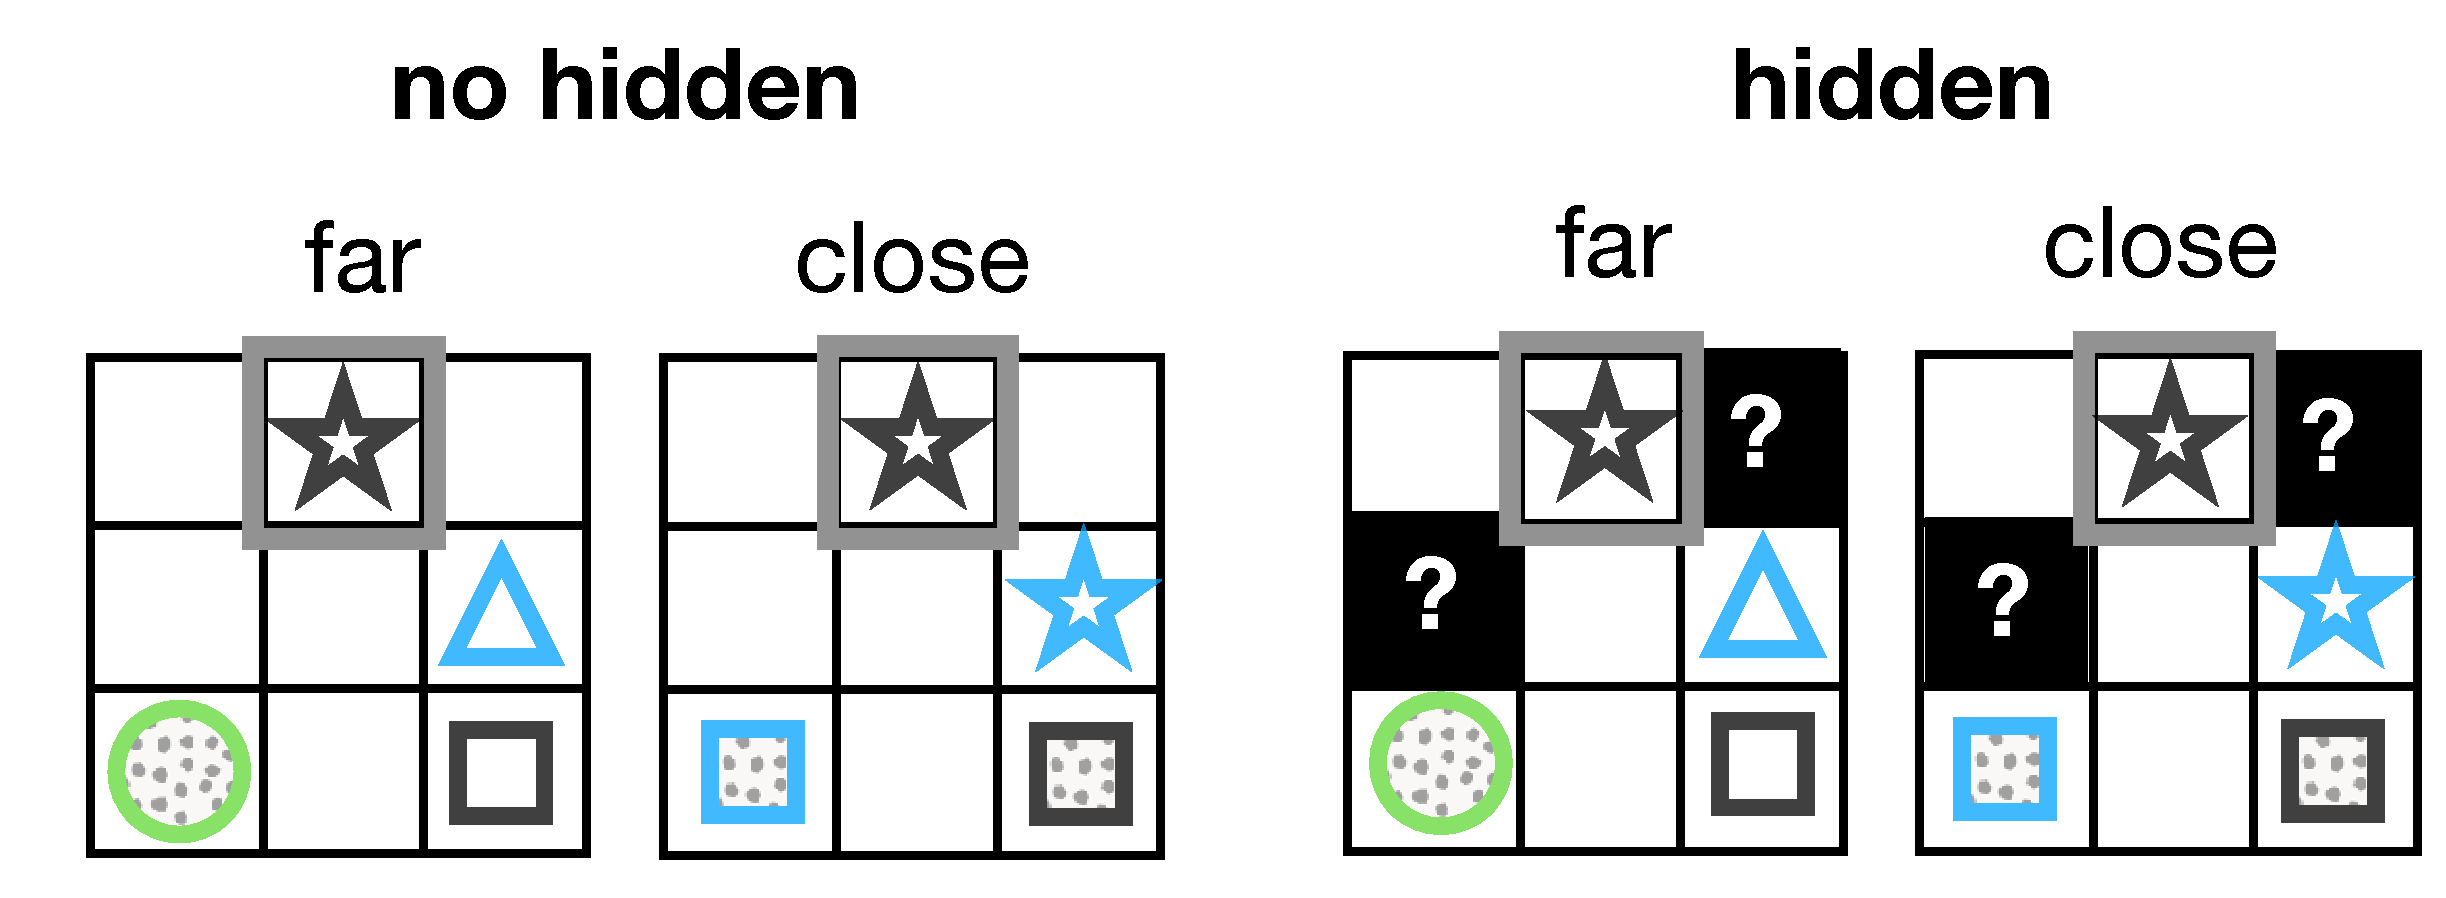
\includegraphics[scale=.3]{figures/Exp2_design}
 \caption{Within-pair factorial design used in Exp.~2. In the common condition, we reproduce a simple pragmatic reference contrast: when more than one star is present in common ground, speakers are expected to be more informative. On hidden versions of these condition, the same set of objects is visible, but some additional squares are occluded. If pragmatic directors represent uncertainty over what the matcher sees behind these squares, we predict that they will produce more informative utterances.}
 \vspace{-.5cm}
 \label{fig:hover}
 \end{center}
 \end{figure}

\subsection{Experiment~2: Production in uncertain contexts}
\label{sec:Exp2}

\subsection{Participants}

We recruited K participants (K/2 pairs) from Amazon Mechanical Turk. All participants were native English speakers. %Three pairs were excluded for making 2 or more errors on non-critical items.

\subsection{Materials \& Procedure}

To more directly test speaker behavior across different contexts, we moved to a more systematic stimulus domain. These objects varied along three discrete features: \emph{shape}, \emph{texture}, and \emph{color}. Each feature took four discrete values, giving a space of 64 possible objects. We placed these objects in a smaller $3 \times 3$ grid, and used a pure \emph{reference game} setup where listeners had to click the intended referent as opposed to following a movement instruction. 

To test how speakers flexibly modify their informativity in response to the uncertainty posed by 

\section{Evaluating models of referring}

\subsection{Pure egocentrism}

The simplest strategy for a speaker attempting to refer to a target object $o_i$ is to produce the simplest label that best fits $o_i$, effectively ignoring context and listener knowledge. \todo[inline]{rxdh: technically, mean soft-max here...} Similarly, the simplest strategy for a listener is to pick the object in their view that is best described by the utterance, ignoring the visual access or pragmatic goals of the speaker. These models are purely egocentric, in the sense that they do not engage in any social reasoning. 

\subsection{Pure consideration of visual access}

The most immediate model of social reasoning is consideration of the informativeness of a label in a shared context containing many objects. For a speaker, this means preferring labels that are good fits for the target but \emph{not} known distractors in common view. For instance, when referring to a dog in the shared context of other dogs, a speaker may opt to be more informative than simply saying `dog,' since it is ambiguous. For a listener, this means discounting objects that are not in shared context, regardless of how well the description fits. These are not available to the visual access of the speaker and thus not viable referents. 

\subsection{Probabilistic weighing of perspectives}

Rather than taking a purely egocentric perspective or purely considering a partner's visual access, speakers or listeners may be probabilistically integrating these two perspectives \cite{HellerParisienStevenson16_ProbabilisticWeighing}. % When conversational expectations lead participants to expect over-informative utterances, they (rationally) place relatively less weight on features of the environment determining common ground, such as shared perceptual access. 

\subsection{Gricean communication under uncertainty}

We begin by considering the problem faced by a speaker who wants their partner to select a target object from a context containing other potentially similar objects. %  a simple probabilistic model of reference in the rational speech act (RSA) model. 

where speakers produce informative utterances by reasoning about a rational listener agent who updates their beliefs about the world according to the literal semantics of the language. This allows us to test pragmatic accounts of task performance. 

Pragmatic critiques of the director-matcher task point to an additional source of uncertainty that has not previously been explored: uncertainty over a communication partner's visual context. Considering this uncertainty, of course, \emph{is} theory of mind in action; our goal is to show how such a model built on social reasoning can produce the `failures' found by \cite{KeysarLinBarr03_LimitsOnTheoryOfMindUse} as well as the phenomena observed by both \cite{HawkinsGoodman16_Keysar} and \cite{RubioFernandez16_DirectorTaskAttention}. For simplicity, we consider the full $2\times 2$ grid containing a single occluded cell, which was used by \cite{RubioFernandez16_DirectorTaskAttention}. We incorporate this source of uncertainty into both the speaker and listener models as follows:

\begin{enumerate}
\item A pragmatic speaker perceives an array of three objects $\mathcal{O}_S = \{o_i\}$, one of which is identified as a target $t$, but assumes that their partner sees an additional hidden object $o_h$ that is not in common ground. The speaker has uncertainty over the identity of this object, represented by a prior distribution $P(o_h)$ which they marginalize over when deciding what utterance to produce:
$$S_1(u | t, \mathcal{O}_p) \propto \sum_{o_h} L_0(t| \mathcal{O}_S \cup \{o_h\})P(o_h)P(u)$$

\item A pragmatic listener, reasoning about this uncertain speaker, is presented with a full array of four objects $\mathcal{O}_L$, one of which is identified as hidden to the speaker, $o_h$. The listener, however, also has some uncertainty over whether the experimenter is deceptive, represented by a Bernoulli random variable $d$, such that they assign a small prior probability $P(d)$ to the possibility that $o_h$ is actually in common ground. Upon hearing an utterance$u$, they update both their beliefs about which object is the target and whether the experimenter is being deceptive:
$$L_2(t, d | u, \mathcal{O}_L) = P(t)\left(S(u | t, \mathcal{O}_L)P(d)\right)^d(S(u | t, \mathcal{O}_L - o_h)(1-P(d))^{1-d}$$
\end{enumerate}
Technical details are omitted here for brevity, but the full model is fully specified in WebPPL and available to run at %\url{http://forestdb.org/models/keysar.html}. 

%We focus on two critical patterns of results produced by the pragmatic listener $L_2$. First, we consider how it responds to the scripted instruction ``fish'' when presented with a context containing two fish (a red one that is occluded and a blue one in common ground) as well as two other unrelated objects. While it is most likely to choose the red fish in common ground, it has a relatively high probability (43\%) of choosing the hidden red fish, an effect \cite{KeysarLinBarr03_LimitsOnTheoryOfMindUse} claimed was due to failure of theory of mind. This decision emerges in the model for two primary reasons. For one, a speaker with uncertainty over context could in principle be communicating about any object, and if they believed the hidden object was a red fish, the utterance `fish' would have a high probability of being produced. To a lesser extent, context uncertainty makes the overinformative utterance `blue fish' more likely than `fish', hence the omission of the color modifier has the (subtle) implication of \emph{not} the blue fish. This speaker phenomenon, while subtle under the parameter regime of the current implementation, produces the dynamic observed in the unscripted replication by  \cite{HawkinsGoodman16_Keysar}.
%
%Second, we consider the listener's posterior over the \emph{deception} Bernoulli variable $d$. Just as \cite{RubioFernandez16_DirectorTaskAttention} found that listeners were more likely to suspect deception after hearing an `overinformative' utterance like `blue fish' when only one fish was in common ground, so too does our pragmatic listener. The pragmatic speaker is relatively more likely to produce the additional color modifier if they see multiple fish than when they see a single fish and simply have uncertainty over the unknown object. Hence, our model simultaneously captures all three phenomena. 

\section{General Discussion}

Pragmatic language understanding requires sophisticated social reasoning. To interpret an utterance, a listener must consider how a speaker is likely to behave in context.
The rational use of theory of mind for a listener thus depends on her expectations about the speaker: If, in a particular context, she expects a speaker to provide sufficiently informative utterances, she may be justified in neglecting his epistemic state when resolving reference.

%consider the speaker's communicative goals and context. 
In our replication (Expt.~1), we found evidence that listeners neglect the speaker's epistemic state, as Keysar and colleagues claim.
We also found that when the speaker's utterance fit the hidden distractor better than the target, matchers were more likely to make errors. 
Indeed, we found that the extremely heterogeneous pattern of errors across items was well explained by the relative fit of the utterance to target and distractor.
This suggests that reference disambiguation was driven primarily by \emph{a priori} label fitness rather than consideration of occluded vs. mutual visible items. 
%
However, this does not necessarily imply limitations on theory of mind---if speakers could be expected to naturally provide expressions which apply better to the target, then this behavior would be appropriate.
% If listeners arrive at this interpretation strategy through pragmatic reasoning, then neglecting the speaker's epistemic state would be rational and also the result of theory of mind use. 
In Expt.~2, we found that speakers did naturally produce more precise, informative utterances than required and these unconstrained utterances fit the target significantly better than they fit the hidden distractor. 
For example, no speaker in Expt.~2 produced ``the bottom block,'' which was used as a critical instruction in Expt.~1. Instead, they said ``the bluish block with a B'' or ``block with the blue writing,'' which relied on less confusable perceptual features and thereby decreased error rates. 
Thus, the errors observed in Expt.~1 can be explained as a result of an uncooperative confederate (speaker)---the experiment set up certain pragmatic expectations through the task context, then deliberately flouted them in critical trials. 

The Gricean maxim of quality dictates that cooperative speakers should make their utterance as informative as is required for current purposes, but no more so. If the referring expressions used in Expt.~1 uniquely pick out the target from the speaker's perspective, then why would unscripted speakers in Expt.~2 be more informative than this? 
%strictly necessary and why would listeners come to expect such ``overinformativity''? 
One possibility is that awareness of the complex mismatch in epistemic state with the listener leads the speaker to provide extra information in an attempt to avoid miscommunication.
Another possibility is that more general dynamics of language are in play.
Studies of over-informativity in referring expressions have uncovered a general tendency of speakers to provide redundant information.
This tendency can depend on a number of situational factors, such as the tendency to mention perceptually salient features to speed up the identification process  \cite{KoolenGattGoudbeekKrahmer11_Overspecification}. 
%In the current task, it seems particularly relevant that both participants knew about the presence of hidden objects, increasing uncertainty about possible distractors and placing additional pressure on the speaker to overspecify. 
The exact origin is a subject that must be followed up by future research \cite[e.g.]{GannBarr14_AudienceDesign}, but it is clear that the tendency of speakers to produce highly informative referring expressions is useful to, and relied on by, listeners. 
%Indeed, the remaining errors in Expt.~2 are at least partially due to the lack of availability of more specific expressions. 
%The items on which errors were most likely in Expt.~2 were difficult precisely because the natural utterance was \emph{still} ambiguous: even if the speaker uses ``hairbrush'' instead of the basic-level ``brush,'' for example, the distractor remains a more typical exemplar of the subcategory.

Further work in a wider variety of tasks is necessary to pin down the various factors determining the relative weighting of these different sources of information, but we have argued that pragmatics play a crucial role.

Previous theoretical advances in modeling pragmatics have typically hinged on `lifting' inference over some aspect of communication that was previously assumed to be fixed. For instance, \emph{manner implicatures} emerge from uncertainty over the true meanings of words in the lexicon \cite{BergenLevyGoodman16_LexicalUncertainty}, nonliteral constructions like \emph{hyperbole} and \emph{irony} emerge from uncertainty over the topic of discussion \cite{KaoWuBergenGoodman14_NonliteralNumberWords}, and \emph{prosody} and \emph{ellipsis} emerge from uncertainty (in the form of a noisy-channel model) over the various ways that a speaker's utterance could have been corrupted  \cite{BergenGoodman15_StrategicUseOfNoise}. Note that these are not ad hoc extensions; sources of uncertainty that are not strictly necessary to explain a particular effect are often omitted for simplicity, but they all coexist within the same model. 

% While We expect our conversation partners to follow common conventions about the meanings of words \cite{Lewis69_Convention, CentolaBaronchelli15_ConventionEmergence}, to update these conventions in light of previous interactions \cite{BrennanClark96_ConceptualPactsConversation}, and perhaps most importantly, 

It is worth noting several significant differences between our study and \cite{KeysarLinBarr03_LimitsOnTheoryOfMindUse}.
The primary difference between our study and the original, of course, is that it was run on the web with participants connected through a virtual environment, instead of face-to-face in a room. We believe we addressed the major concern about exploring theory of mind in web experiments -- that participants do not truly believe they are interacting with another human -- by allowing instantaneous, responsive, real-time interaction.  On the other hand, it is known that textual communication, as in our chat box, can differ from face-to-face verbal communication. Additionally, we omitted the procedural step of placing the hidden distractor in a paper bag, and some aspects of the interface such as the graphical representation of occluded cells may be less intuitive, or require more training, on the web than in the lab. % Directors watched objects move through the actual moment-by-moment mouse trajectories that matchers used to drag them, and matchers saw the actual timing of the messages sent by the director.

A related difference is our decision not to use a confederate. While confederates are useful for reducing variation across instances of the experiment and delivering carefully targeted manipulations, their use may have unexpected consequences. Beyond the difficulties of conducting large-scale experiments with confederates, it is difficult to exactly replicate all the subtleties of the confederate's behavior that might influence results. The pair of experiments we report is a reminder that manipulations administered by a trained confederate can interact in unexpected ways with a participant's social and communicative expectations. Regardless of the experimental context, it is illuminating to see how real participants naturally interact.

\todo[inline]{mention rubio fernandez early?}
Using similar reasoning, \cite{RubioFernandez16_DirectorTaskAttention} showed that listeners became suspicious of what was actually in common ground after hearing overinformative utterances, thus successfully using theory of mind reasoning. 

\todo[inline]{Mention Westra \& Carruthers as another critique focusing on pragmatics?}

\todo[inline]{Mention neural coordination papers? e.g. Stephens et al 2010, Stolk et al, 2014?}

%
%\section{Sample Section}
%Text here. Text here. Text here. Text here.
%Text here. Text here. Text here. Text here.
%Text here. Text here. Text here. Text here.
%Text here. Text here. Text here. Text here.
%
%\subsection{Sample Subsection}
%Text here. Text here. Text here. Text here.
%Text here. Text here. Text here. Text here.
%Text here. Text here. Text here. Text here.
%Text here. Text here. Text here. Text here.
%
%\subsubsection{Sample Subsubsection}
%Text here. Text here. Text here. Text here.
%Text here. Text here. Text here. Text here.
%Text here. Text here. Text here. Text here.
%Text here. Text here. Text here. Text here.
%
%\section{Sample equations}
%\begin{equation}
%\label{eq:rhoCHT}
%\rho^{\pi}= \frac{RI + \mathbb{E}_{\pi([L,\tau_L]|\textrm{post})}
%\left[C_L(\taupav+\tau_L) \right]   +
%\displaystyle{\int_{0}^{P}}{dw~ \mathbb{E}_{\pi_{w_L}}}
%\Biggl[\/\sum_{n_{L|[\textrm{pre},w]}}C_L(\tau_L)
%\Biggr]            }      {P +
%\mathbb{E}_{\pi([L,\tau_L] |\textrm{post})}[\tau_{L}] +\taupav +
%\displaystyle{ \int_{0}^{P}}{dw~ \mathbb{E}_{\pi_{w_L}}}   
%\Biggl[\sum_{n_{L|[\textrm{pre},w]}}\tau_L\Biggr]  
%}
%\end{equation}
%As long as
%$RI - K_LP > 
%\frac{1}{\beta}$
%\begin{equation}
%%\def\theequation{5.1}
%\left.\begin{array}{lrcl}
%&\rho^{\pi} &=&  \displaystyle\frac{\beta ( RI + K_L \taupav )-1} {\beta
%(P+\taupav )}    \\[12pt]
%\hbox{and}\hbox to .25in{\hfill}&\mathbb{E}[\tau_L | \text{post}] &=&\displaystyle \frac{P+\taupav}{\beta ( RI -
%K_LP)-1}  
%\label{eq:analytical_linear}
%\end{array}\right\}\hbox to 1.25in{\hfill}
%\end{equation} 
%
%\subsection{Simple code sample}
%
%\begin{code}
%\begin{verbatim}
%procedure bubbleSort( A : list of sortable items )
%    n = length(A)
%    repeat
%       newn = 0
%       for i = 1 to n-1 inclusive do
%          if A[i-1] > A[i] then
%             swap(A[i-1], A[i])
%             newn = i
%          end if
%       end for
%       n = newn
%    until n = 0
%end procedure
%\end{verbatim}
%\end{code}
%
%
%
%\subsection{Algorithm environment}
%
%%% \begin{algorithm} takes option [p][b][t][h],  or some combination, like \begin{figure}
%%% See documentation for algorithmic.sty for more information on formatting algorithms.
%
%\begin{algorithm}[h]
%\caption{A sample in an algorithm environment.}
%\begin{algorithmic}
%\If {$i\geq maxval$}
%    \State $i\gets 0$
%\Else
%    \If {$i+k\leq maxval$}
%        \State $i\gets i+k$
%    \EndIf
%\EndIf
%\end{algorithmic}
%\end{algorithm}
%
%
%\section{Jargon definitions}
%
%\begin{wideboxedtext}
%\begin{glossary}
%\symbol{Term} Definition
%\symbol{Term} Definition
%%ie
%%\symbol{$1/\lambda$} mean of exponential effective prior probability density for leisure time
%%\symbol{CHT} Cumulative Handling Time 
%\end{glossary}
%\end{wideboxedtext}
%
%\begin{boxedtext}
%\begin{glossary}
%\symbol{Term} Definition
%\symbol{Term} Definition
%%ie
%%\symbol{$1/\lambda$} mean of exponential effective prior probability density for leisure time
%%\symbol{CHT} Cumulative Handling Time 
%\end{glossary}
%\end{boxedtext}
%
%\section{Itemized Lists}
%
%\subsection{Roman list:}
%
%\begin{enumerate}
%\item[(i)] at high 
%payoffs, subjects work almost continuously, engaging in little leisure
%in between work bouts; 
%\item[(ii)] at low payoffs, they 
%engage in leisure all at once, in long bouts after working, rather
%than distributing the same amount of leisure time into multiple short
%leisure bouts; 
%\item[(iii)] subjects work continuously for the entire price duration, as long as
%the price is not very long (as shown by an analysis conducted by Y-AB, to be published separately); %(\textbf{Figure \ref{fig:task_data}D}).
%\item[(iv)] the duration of leisure bouts is variable.
%\end{enumerate}
%
%\subsection{Numbered list:}
%
%\begin{enumerate}
%\item at high 
%payoffs, subjects work almost continuously, engaging in little leisure
%inbetween work bouts; 
%\item at low payoffs, they 
%engage in leisure all at once, in long bouts after working, rather
%than distributing the same amount of leisure time into multiple short
%leisure bouts; 
%\item subjects work continuously for the entire price duration, as long as
%the price is not very long (as shown by an analysis conducted by Y-AB, to be published separately); %(\textbf{Figure \ref{fig:task_data}D}).
%\item the duration of leisure bouts is variable.
%\end{enumerate}
%
%
%\subsection{Bulleted list:}
%
%\begin{itemize}
%\item at high 
%payoffs, subjects work almost continuously, engaging in little leisure
%inbetween work bouts; 
%\item at low payoffs, they 
%engage in leisure all at once, in long bouts after working, rather
%than distributing the same amount of leisure time into multiple short
%leisure bouts; 
%\item subjects work continuously for the entire price duration, as long as
%the price is not very long (as shown by an analysis conducted by Y-AB, to be published separately); %(\textbf{Figure \ref{fig:task_data}D}).
%\item the duration of leisure bouts is variable.
%\end{itemize}
%
%
%\section{Sample citations}
%For general information on the correct form for citations using
%the APA 6 format, see the following sites:
%\href{https://owl.english.purdue.edu/owl/resource/560/02/}
%{APA 6, In-text citations, The Basics} and
%\href{https://owl.english.purdue.edu/owl/resource/560/03/}
%{APA 6, In-text citations}
%
%\section{Natbib citation mark up}
%
%\subsection{Single citations}
%\noindent
%\begin{tabular}{ll}
%\bf Type&\bf Results\\
%\hline
%\verb+\citet{jon90}+&Jones et al. (1990)\\
%\verb+\citet[chap. 2]{jon90}+&Jones et al. (1990, chap. 2)\\
%    \verb+\citep{jon90}+	    &   	(Jones et al., 1990)\\
%    \verb+\citep[chap. 2]{jon90}+ 	&    	(Jones et al., 1990, chap. 2)\\
%    \verb+\citep[see][]{jon90}+ 	 &    	(see Jones et al., 1990)\\
%    \verb+\citep[see][chap. 2]{jon90}+ 	&    	(see Jones et al., 1990, chap. 2)\\
%    \verb+\citet*{jon90}+ 	    &    	Jones, Baker, and Williams (1990)\\
%    \verb+\citep*{jon90}+	    &    	(Jones, Baker, and Williams,
%    1990) \\
%\end{tabular}
%
%For example, some citations from the OpenMindSample bibliography:
%citet:\citet{anderson}, citep:\citep{antibayes}, and
%cite*: \citet*{anderson}.
%
%\subsection{Multiple citations}
%Multiple citations may be made by including more than one citation
%key in the \verb+\cite+ command argument.
%
%\noindent
%\begin{tabular}{ll}
%\bf Type&\bf Results\\
%\hline
%\verb+\citet{jon90,jam91}+&Jones et al. (1990); James et al. (1991)\\
%\verb+\citep{jon90,jam91}+&(Jones et al., 1990; James et al. 1991)\\
%\verb+\citep{jon90,jon91}+&(Jones et al., 1990, 1991)\\
%\verb+\citep{jon90a,jon90b}+&(Jones et al., 1990a,b)\\
%\end{tabular}
%
%For example, multiple citations from the OpenMindSample bibliography:
%citet:\citet{anderson,antibayes}, citep:\citep{anderson,antibayes}.
%As you see, the citations are automatically hyperlinked to their
%reference in the bibliography.
%
%\newpage
%
%\section{Sample figures}
%
%\begin{figure}[h] 
%\centerline{\includegraphics[width=\textwidth]{Fig1}}
%\caption{(Colour online) \textbf{Task and key features of the
% data.} \\
% A) Cumulative handling time (CHT) task. Grey bars denote work
%(depressing a lever), white gaps show leisure. The subject must
% accumulate work up to a total period of time called the
%\emph{price} ($P$) in order to obtain a single reward (black dot) of subjective reward
%intensity $RI$. The trial duration is $25\times \mathrm{price}$ (plus
%$2$s each time the price is attained, during which the lever is retracted so it cannot
%work; not shown).
%}
%\label{fig:task_data}
%\end{figure}
%
%\begin{figure}[ht] 
%\widefigure{\fullpagewidth}{Fig1}
%\caption{(Colour online) \textbf{Task and key features of the
% data.} \\
%A) Cumulative handling time (CHT) task. Grey bars denote work
%(depressing a lever), white gaps show leisure. The subject must
%accumulate work up to a total period of time called the
%\emph{price} ($P$) in order to obtain a single reward (black dot) of subjective reward
%intensity $RI$. The trial duration is $25\times \mathrm{price}$ (plus
%$2$s each time the price is attained, during which the lever is retracted so it cannot
%work; not shown).
%}
%\label{newfig:task_data}
%\end{figure}
%
%\clearpage
%\section{Sample tables}
%
%\begin{table}[!ht]
%\caption{Time of the Transition Between Phase 1 and Phase 2$^{a}$}
%\label{tab:label}
%\centering
%\begin{tabular}{lc}
%\hline
% Run  & Time (min)  \\
%\hline
%  $l1$  & 260   \\
%  $l2$  & 300   \\
%  $l3$  & 340   \\
%  $h1$  & 270   \\
%  $h2$  & 250   \\
%  $h3$  & 380   \\
%  $r1$  & 370   \\
%  $r2$  & 390   \\
%\hline
%\multicolumn{2}{l}{$^{a}$Table note text here.}
%\end{tabular}
%\end{table}
%
%\begin{table}[ht]
%\widecaption{Sample table taken from [treu03]\label{tbl-1}}
%\begin{widetable}
%\advance\tabcolsep-1pt
%\small
%\begin{tabular}{ccrrccccccccc}
%\hline
%\bf 
%POS &\bf  chip &\multicolumn1c{\bf ID} &\multicolumn1c{\bf X}
%&\multicolumn1c{\bf Y} &\bf
%RA &\bf DEC &\bf IAU$\pm$ $\delta$ IAU &\bf
%IAP1$\pm$ $\delta$ IAP1 &\bf IAP2 $\pm$ $\delta$
%IAP2 &\bf star &\bf E &\bf Comment\\
%\hline
%0 & 2 & 1 & 1370.99 & 57.35\rlap{$^a$}    &   6.651120 &  17.131149 &
%21.344$\pm$0.006\rlap{$^b$}  & 2 4.385$\pm$0.016 & 23.528$\pm$0.013 & 0.0 & 9 & -    \\
%0 & 2 & 2 & 1476.62 & 8.03     &   6.651480 &  17.129572 & 21.641$\pm$0.005  & 2 3.141$\pm$0.007 & 22.007$\pm$0.004 & 0.0 & 9 & -    \\
%0 & 2 & 3 & 1079.62 & 28.92    &   6.652430 &  17.135000 & 23.953$\pm$0.030  & 2 4.890$\pm$0.023 & 24.240$\pm$0.023 & 0.0 & - & -    \\
%0 & 2 & 4 & 114.58  & 21.22    &   6.655560 &  17.148020 & 23.801$\pm$0.025  & 2 5.039$\pm$0.026 & 24.112$\pm$0.021 & 0.0 & - & -    \\
%0 & 2 & 5 & 46.78   & 19.46    &   6.655800 &  17.148932 & 23.012$\pm$0.012  & 2 3.924$\pm$0.012 & 23.282$\pm$0.011 & 0.0 & - & -    \\
%0 & 2 & 6 & 1441.84 & 16.16    &   6.651480 &  17.130072 & 24.393$\pm$0.045  & 2 6.099$\pm$0.062 & 25.119$\pm$0.049 & 0.0 & - & -    \\
%0 & 2 & 7 & 205.43  & 3.96     &   6.655520 &  17.146742 & 24.424$\pm$0.032  & 2 5.028$\pm$0.025 & 24.597$\pm$0.027 & 0.0 & - & -    \\
%0 & 2 & 8 & 1321.63 & 9.76     &   6.651950 &  17.131672 &
%22.189$\pm$0.011  & 2 4.743$\pm$0.021 & 23.298$\pm$0.011 & 0.0 & 4 &
%edge \\
%\hline
%\multicolumn{13}{l}{%
%Table 2 is published in its entirety in the electronic
%edition of the {\it Astrophysical Journal}.}\\[3pt]
%\multicolumn{13}{l}{%
%$^a$ Sample footnote for table 2.}\\[3pt]
%\multicolumn{13}{l}{%
%$^b$ Another sample footnote for table 2.}
%\end{tabular}
%\end{widetable}
%\end{table}
%
%\begin{table}[p]
%\rotatebox{90}{\vbox{\hsize=\textheight
%\caption{Here is a caption for a table that is found in landscape
%mode.}
%\begin{tabular}{ccrrccccccccc}
%\hline
%\bf 
%POS &\bf  chip &\multicolumn1c{\bf ID} &\multicolumn1c{\bf X}
%&\multicolumn1c{\bf Y} &\bf
%RA &\bf DEC &\bf IAU$\pm$ $\delta$ IAU &\bf
%IAP1$\pm$ $\delta$ IAP1 &\bf IAP2 $\pm$ $\delta$
%IAP2 &\bf star &\bf E &\bf Comment\\
%\hline
%0 & 2 & 1 & 1370.99 & 57.35\rlap{$^a$}    &   6.651120 &  17.131149 &
%21.344$\pm$0.006\rlap{$^b$}  & 2 4.385$\pm$0.016 & 23.528$\pm$0.013 & 0.0 & 9 & -    \\
%0 & 2 & 2 & 1476.62 & 8.03     &   6.651480 &  17.129572 & 21.641$\pm$0.005  & 2 3.141$\pm$0.007 & 22.007$\pm$0.004 & 0.0 & 9 & -    \\
%0 & 2 & 3 & 1079.62 & 28.92    &   6.652430 &  17.135000 & 23.953$\pm$0.030  & 2 4.890$\pm$0.023 & 24.240$\pm$0.023 & 0.0 & - & -    \\
%0 & 2 & 4 & 114.58  & 21.22    &   6.655560 &  17.148020 & 23.801$\pm$0.025  & 2 5.039$\pm$0.026 & 24.112$\pm$0.021 & 0.0 & - & -    \\
%0 & 2 & 5 & 46.78   & 19.46    &   6.655800 &  17.148932 & 23.012$\pm$0.012  & 2 3.924$\pm$0.012 & 23.282$\pm$0.011 & 0.0 & - & -    \\
%0 & 2 & 6 & 1441.84 & 16.16    &   6.651480 &  17.130072 & 24.393$\pm$0.045  & 2 6.099$\pm$0.062 & 25.119$\pm$0.049 & 0.0 & - & -    \\
%0 & 2 & 7 & 205.43  & 3.96     &   6.655520 &  17.146742 & 24.424$\pm$0.032  & 2 5.028$\pm$0.025 & 24.597$\pm$0.027 & 0.0 & - & -    \\
%0 & 2 & 8 & 1321.63 & 9.76     &   6.651950 &  17.131672 &
%22.189$\pm$0.011  & 2 4.743$\pm$0.021 & 23.298$\pm$0.011 & 0.0 & 4 &
%edge \\
%\hline
%\multicolumn{13}{l}{%
%Table 2 is published in its entirety in the electronic
%edition of the {\it Astrophysical Journal}.}\\[3pt]
%\multicolumn{13}{l}{%
%$^a$ Sample footnote for table 2.}\\[3pt]
%\multicolumn{13}{l}{%
%$^b$ Another sample footnote for table 2.}
%\end{tabular}
%}}
%\end{table}
%\clearpage
%
%
%\vglue 3in
%Example of table continuing over pages:
%
%
%\begin{center}
%\begin{longtable}{ccc@{}}
%\caption{ApJ costs from 1991 to 2013
%\label{tab:table}} \\[2pt]
%\hline
%\bf Year & \bf Subscription & \bf Publication \\
% & \bf cost &\bf charges\\
% & \bf(\$) & \bf (\$/page)\\
%\hline
%\endfirsthead
%
%\multicolumn3c{Table \thetable, \it continued from previous page.}\\[6pt]
%\multicolumn3c{ApJ costs from 1991 to 2013}\\[2pt]
%\hline
%\bf Year & \bf Subscription & \bf Publication \\
% & \bf cost &\bf charges\\
% & \bf(\$) & \bf (\$/page)\\
%\hline
%\endhead
%\\\hline
%\\[-8pt]
%\multicolumn{3}{r}{\it Table continued on next page}\\ 
%\endfoot
%
%\hline
%\endlastfoot
%
%1991 & 600 & 100 \\
%1992 & 650 & 105 \\
%1993 & 550 & 103 \\
%1994 & 450 & 110 \\
%1995 & 410 & 112 \\
%1996 & 400 & 114 \\
%1997 & 525 & 115 \\
%1998 & 590 & 116 \\
%1999 & 575 & 115 \\
%2000 & 450 & 103 \\
%2001 & 490 &  90 \\
%2002 & 500 &  88 \\
%2003 & 450 &  90 \\
%2004 & 460 &  88 \\
%2005 & 440 &  79 \\
%2006 & 350 &  77 \\
%2007 & 325 &  70 \\
%2008 & 320 &  65 \\
%2009 & 190 &  68 \\
%2010 & 280 &  70 \\
%2011 & 275 &  68 \\
%2012 & 150 &  56 \\
%2013 & 140 &  55 \\
%\end{longtable}
%\end{center}

\section{Supportive Information}
Here you enter further sources of information, if desired.

%% A possible entry might be:
% No supportive information is available at this time.


\acknowledgments
Enter your acknowledgments here.

%% ie.,

% The authors thank Laurence Aitchison for fruitful discussions.  RKN
% and PD received funding from the Gatsby Charitable Foundation. Y-AB,
% RBS, KC and PS received funding from Canadian Institutes of Health
% Research grant $MOP74577$,
% Fond de recherche Qu\'{e}bec - Sant\'{e} (Group grant to the Groupe 
% de recherche en neurobiologie comportementale, Shimon Amir, P.I.), and
% Concordia University Research Chair (Tier I). 

\authorcontributions 
Who helped formulate the project, who supplied data, analyses and
experiments, etc.

%% ie.
%% Project was formulated by RKN, PD, PS,
%% based on substantial data, analyses and experiments of Y-AB, KC, RS,
%% PS. RKN, PD formalised the model, RKN implemented and ran the model;
%% RKN analysed the molecular ethogram data; Y-AB formalised and
%% implemented a CTMC model. All authors wrote the manuscript.


%%%%%%%%%%%%%%%%%%%%%%%
%% The bibliography

%% \nocite{*} is used here as a quick way to get every entry  in the .bib file to
%% appear in the bibliography. Normally the bibliography is made using only
%% the bibentries that you cite using \cite{}, or one of the Natbib citation
%% entries, like \citep{}, \citet{} etc.

%\nocite{*}
\bibliography{refs}


\appendix

\section{Sample Appendix Section}
We derive the result in Eq. \eqref{eq:analytical_linear}. We consider a linear $C_L(\tau_L+\taupav)=K_L(\tau_L+\taupav)$, and
make two further 
simplifications: (i) the subject does not
engage in leisure in the pre-reward state (and so works for the whole
price when it works); and (ii) \emph{a priori}, arbitrarily long leisure durations are possible
($\lambda=0$).
Then the reward rate in Eq. \eqref{eq:rhoCHT} becomes
\begin{equation}\label{eq:analyticalrho}
\rho^{\pi}= \frac{\vrule height 10pt width0pt RI + K_L \{~ \mathbb{E}[ \tau_L | \textrm{post} ] + \taupav  \} }
     {P +
\mathbb{E}[ \tau_L | \textrm{post} ] +\taupav  } 
\end{equation} 
As discussed in the \emph{Results} section, the probability of engaging in instrumental leisure in the post-reward state is $\pi([L,\tau_L]
~| \textrm{post}) = \exp\left[-\{\beta (\rho^\pi-K_L) 
 \} \tau_L\right]$, which is an exponential distribution with
mean 
\begin{equation}
\mathbb{E}[\tau_L | \textrm{post}]=\frac{1}{\beta (\rho^\pi-K_L) }
\label{eq:analyticaltauL}
\end{equation}  
Re-arranging terms of this equation,
\begin{equation}\label{eq:rhoversion2}
\rho^{\pi}=\frac{1}{\beta ~\mathbb{E}[\tau_L | \textrm{post}]} +K_L 
\end{equation} 
Equating Eqs. \eqref{eq:analyticalrho} and \eqref{eq:rhoversion2} and solving for the mean instrumental leisure duration $\mathbb{E}[\tau_L | \textrm{post}]$, we derive
\begin{equation}
\mathbb{E}[\tau_L | \textrm{post}] = \frac{P+\taupav}{\beta ( RI - K_LP)-1} 
\label{eq:solvedtauL}
\end{equation}
which is the second line of Eq.\eqref{eq:analytical_linear}. This is the mean instrumental leisure duration as long as  $RI - K_LP>1$, and  $\mathbb{E}[\tau_L | \textrm{post}] \rightarrow \infty$ otherwise. When the former condition holds, we may
substitute Eq. \eqref{eq:solvedtauL} into Eq. \eqref{eq:analyticalrho} and solve for $\rho^{\pi}$

\begin{figure}
\widefigure{\fullpagewidth}{Fig1}
\caption{Sample Appendix Caption. Here is a caption that might
appear in an appendix. It is as wide as the full width of the page.}
\end{figure}

\newpage

\section{Making Your Bibliography for an Open Mind Article}
{\it Open Mind} uses the APA author-date  bibliography style,
apacite.bst. For more
information on apacite, for examples in how to make your .bib file and more, see:\\
\href{http://mirror.jmu.edu/pub/CTAN/biblio/bibtex/contrib/apacite/apacite.pdf}
{http://mirror.jmu.edu/pub/CTAN/biblio/bibtex/contrib/apacite/apacite.pdf}

\noindent
(In spite of the mention of apacite cite commands, please use only
Natbib commands for in text citations, as shown above.)

\subsection{BibTeX}
You will need to use BibTeX to form your bibliography; typing in the
references would be
a huge and unpleasant task. Look at the openmindsample.bbl file and you'll see why
typing in the bibitems would be difficult. 

For a good basic introduction to using BibTeX, see
\href{https://www.economics.utoronto.ca/osborne/latex/BIBTEX.HTM}
{https://www.economics.utoronto.ca/osborne/latex/BIBTEX.HTM}

When you use BibTeX, the form of the bibliography will be correct. You
don't need to supply a bibliography style, since that is built into
the stjour.cls file.

\end{document}

